\documentclass[a4paper,11pt]{scrbook}
\usepackage[utf8]{inputenc}
\usepackage[ngerman]{babel}

\usepackage{setspace}

\usepackage{geometry}
\geometry{top=3.5cm, left=3cm, right=3cm, bottom=3.5cm}

\usepackage{lipsum}
\usepackage{pdfpages}
\usepackage{booktabs}
\usepackage{graphicx}
\usepackage{xcolor}
\usepackage{natbib}

\usepackage{fancyhdr}
\pagestyle{fancy}
\lhead{\thepage}
\rhead{\textit{\nouppercase \leftmark}}
\cfoot{ }

\fancyhead[LE]{\thepage}
\fancyhead[RO]{\emph{\thepage}}
\fancyhead[LO]{\textit{\nouppercase \rightmark}}

\graphicspath{ {pic/} }

\usepackage{caption}
\captionsetup[figure]{format=plain,justification=justified,font={footnotesize},labelfont=bf}

\usepackage{color}
 \definecolor{myblue}{rgb}{0,0,0.40}
 \definecolor{myred}{rgb}{1,0,0}
\usepackage[colorlinks=true,linkcolor=myblue,citecolor=myblue,bookmarks=true,bookmarksopen=true,
	    pdfauthor={Ingo},pdftitle={aufgabe_38},pdfkeywords={Latex,Tex,ASQ,Ingo},
	    pdfsubject={tex},pdfcreator={Ingo},pdfproducer={pdflatex},pdfpagelayout=SinglePage]{hyperref}
	    

\usepackage{ragged2e}

\usepackage{placeins}

\usepackage{natbib}
 \bibliographystyle{unsrtnat}
 \setcitestyle{notesep={; },round,aysep={},yysep={;}}

\title{Titel der Dissertation}
	  


\begin{document}
\frontmatter
\thispagestyle{empty}
\doublespacing
\centering{
\ \\
\ \\
\vspace{1.25cm}
\LARGE{\textbf{Titel der Dissertation}}\\
\vspace{1.6cm}
\Large{\textbf{Dissertation}}\\
\large{\textbf{zur Erlangung des akademischen Grades}}\\
doctor rerum naturalium (Dr. rer. nat.)\\
\textbf{vorgelegt dem Rat der Fakultät für Mathematik und Informatik der Friedrich-Schiller-Universität Jena\\
von} XXX\\
\textbf{am} TT.MM.YYYY \textbf{in} XXX}
\clearpage

\singlespacing
\raggedright
\chapter*{Zusammenfassung}
\justifying
\lipsum[1-7]
\newpage

\chapter*{Danksagung}
\lipsum[1-2]

\tableofcontents

\mainmatter
\chapter{Einleitung}
\lipsum[1-10]
\pagebreak
\chapter{Methoden}


\begin{otherlanguage}{english}
(%
 \glqq Mathematica appears to be like the girl with the little curl right in the middle of her forehead:
 when it is good, it can be very very good, but when it's bad, it can be horrid.\grqq %
)
\end{otherlanguage}
\citep*[p.~12]{Wolfram:91}\\
\lipsum[1-2]
\section{Einfache Methode}
\begin{otherlanguage}{english}
(%
 \glqq Low back pain has major socioeconomic implications; 
 much of the costs relate to disability and compensation. 
 Theoretically, the early identification of patients at risk to become disabled from a low back episode 
 would lead to more aggressive intervention and reduction of subsequent disability.\grqq %
) 
\end{otherlanguage}
\citep*[p.~36]{Frymoyer:87}\\
\lipsum[1-5]

\section{Schwierige Methode}
\begin{otherlanguage}{english}
(%
 \glqq Lipidic NanoCapsules (LNCs) were prepared via an emulsion phase inversion method. 
 Nanoparticles with hydrodynamic diameter of 25, 50 and 100 nm were easily obtained. 
 Their surfaces are covered with short PEG chains (PEG 660) which are not bearing any chemical reactivities.\grqq %
) 
\end{otherlanguage}
\citep*[p.~3]{Perrier:11}\\
\lipsum[1-5]
Quisque facilisis auctor sapien. Pellentesque gravida hendrerit lectus. Mauris
rutrum sodales sapien. Fusce hendrerit sem vel lorem. Integer pellentesque massa vel augue. Integer
elit tortor, feugiat quis, sagittis et, ornare non, lacus.
\begin{figure}[h]

\includegraphics[width=\textwidth]{platzhalter}
\caption[Quisque facilisis auctor sapien.]
{Quisque facilisis auctor sapien. Pellentesque gravida hendrerit lectus. Mauris
rutrum sodales sapien. Fusce hendrerit sem vel lorem. Integer pellentesque massa vel augue. Integer
elit tortor, feugiat quis, sagittis et, ornare non, lacus. Vestibulum posuere pellentesque eros. Quisque
venenatis ipsum dictum nulla. Aliquam quis quam non metus eleifend interdum. Nam eget sapien
ac mauris malesuada adipiscing. Etiam eleifend neque sed quam. Nulla facilisi. Proin a ligula. Sed
id dui eu nibh egestas tincidunt. Suspendisse arcu.} 
\end{figure}
\lipsum[1-5]

\pagebreak
\chapter{Ergebnisse}
\lipsum[1-9]
\pagebreak
\chapter{Schlussfolgerung}
\lipsum[1-4]

\appendix
%\nocite{}
\bibliographystyle{alpha}
\bibliography{buch.bib}

\chapter{Anhang}
\lipsum[1-2]

\backmatter
\listoffigures
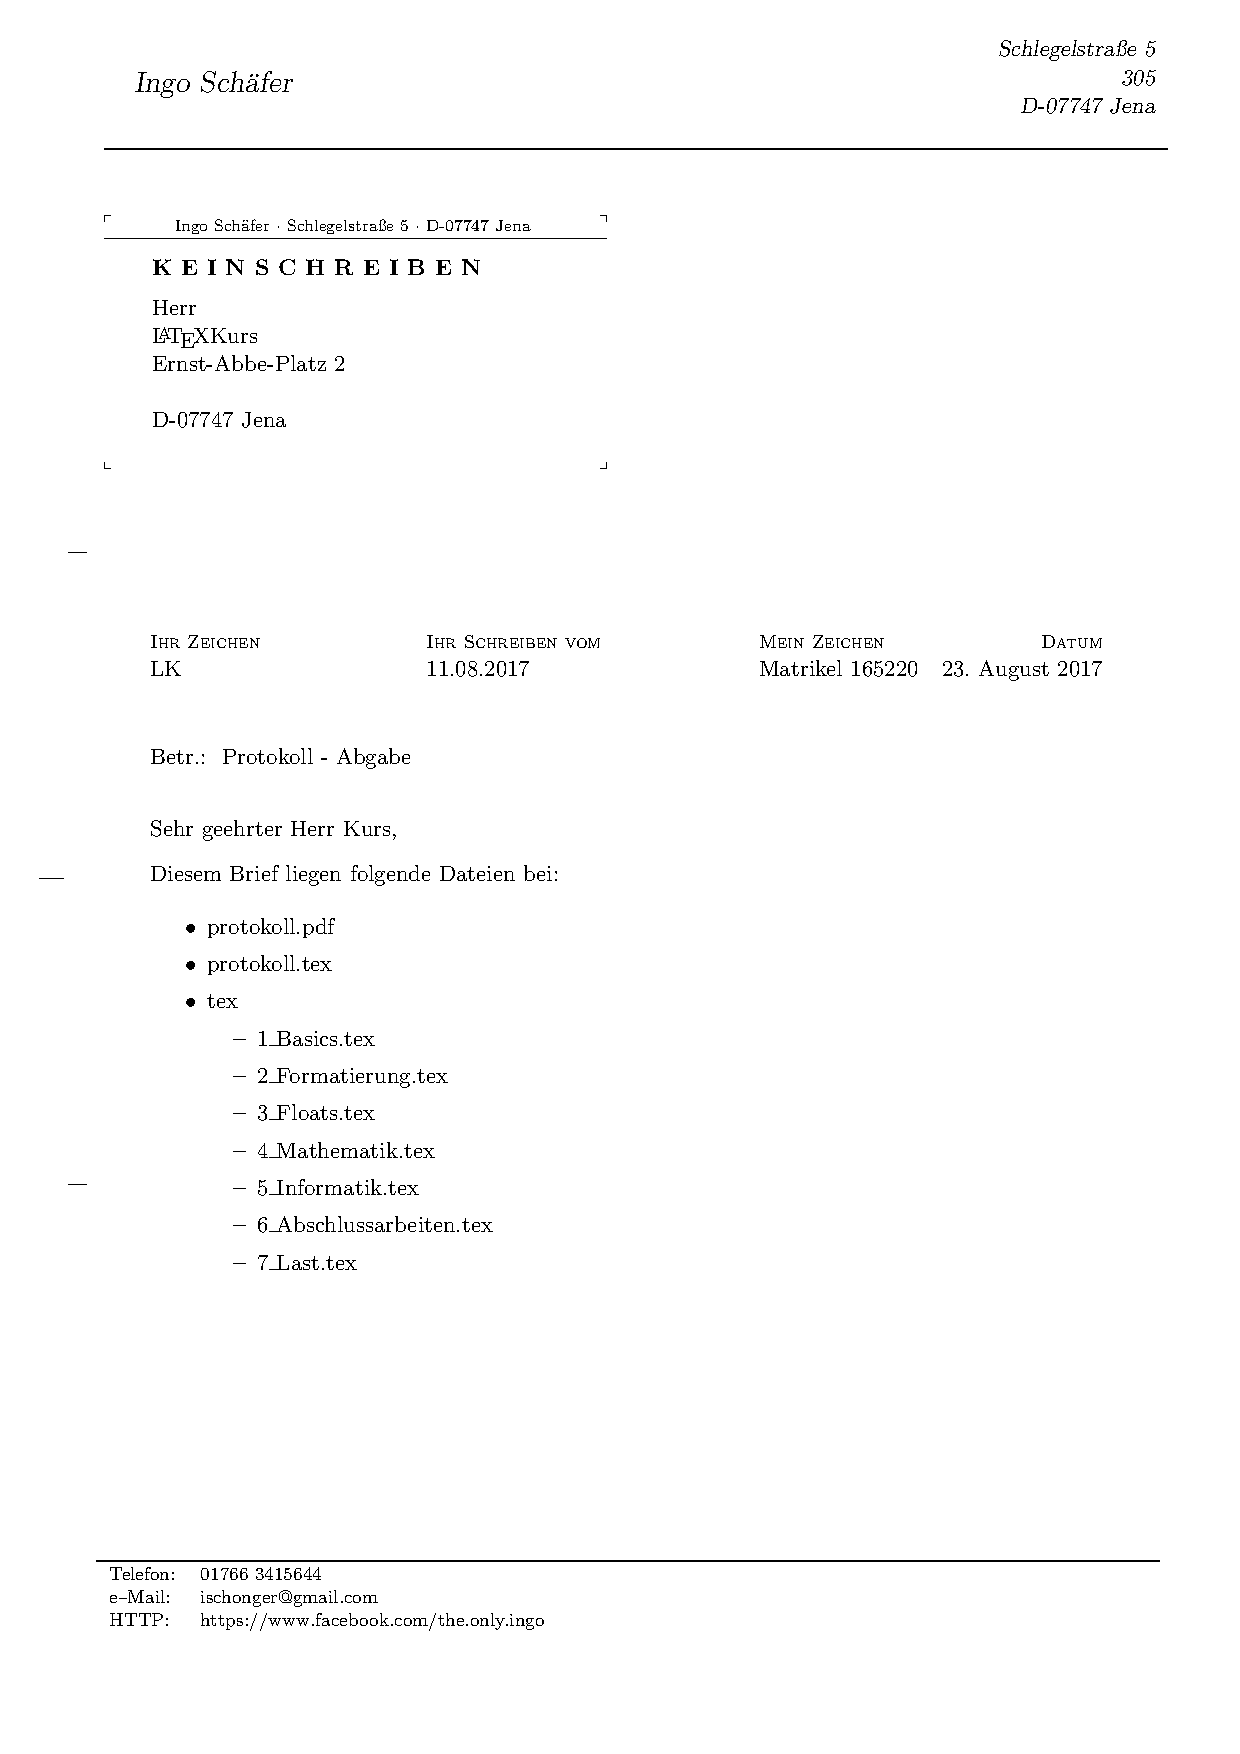
\includepdf[page=4]{../protokoll}


\end{document}